\subsection{D Latch (Transparent Latch)}
\label{subsec:d-latch}

One way to eliminate the undesirable condition of the indeterminate state in the $SR$ latch is to ensure that inputs $S$ and $R$ are never equal to 1 at the same time. This is done in the $D$ latch, shown in Fig. 6. 
\begin{figure}[H]
  \centering
  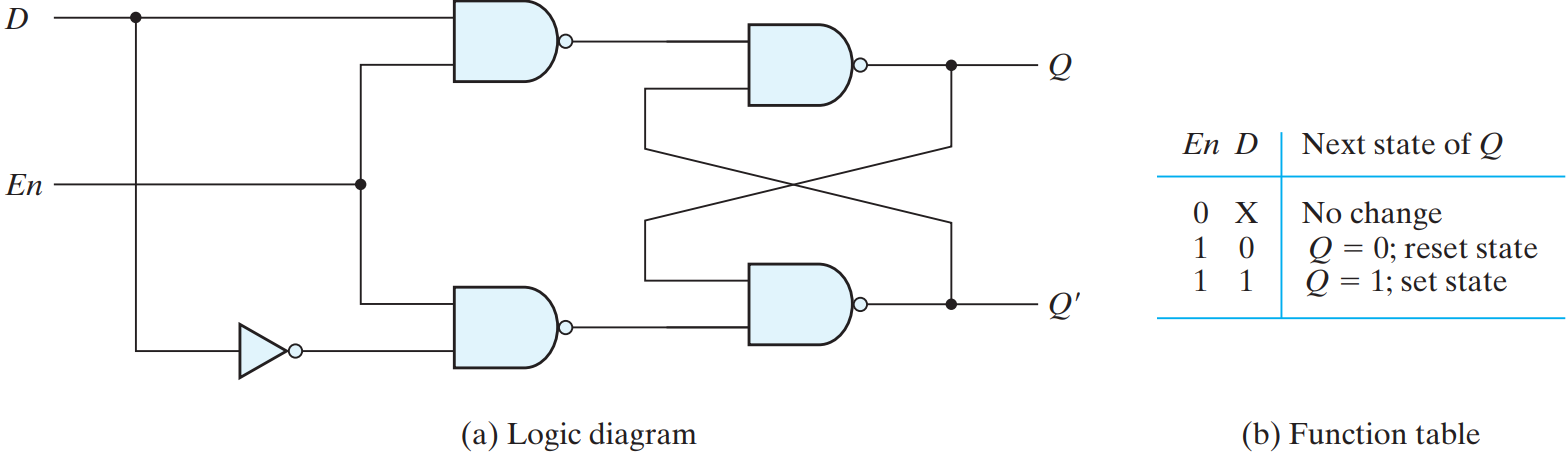
\includegraphics[width=\linewidth]{img/fig-5.6.png}
  \caption{D Latch}
  \label{fig:5.6}
\end{figure}
\noindent This latch has only two inputs: $D$ (data) and $En$ (enable). The $D$ input goes directly to the $S$ input, and its complement is applied to the $R$ input. 

The $D$ latch receives that designation from its ability to hold data in its internal storage. It is suited for use as a temporary storage for binary information between a unit and its environment. The binary information present at the data input of the $D$ latch is transferred to the $Q$ output when the enable input is asserted. The output follows changes in the data input as long as the enable input is asserted.

The circuit is often called a transparent latch. When the enable input signal is de-asserted, the binary information that was present at the data input at the time the transition of enable occurred is retained (i.e., stored) at the $Q$ output until the enable input is asserted again.

The graphic symbols for the various latches are shown in Fig. 7.
\begin{figure}[H]
  \centering
  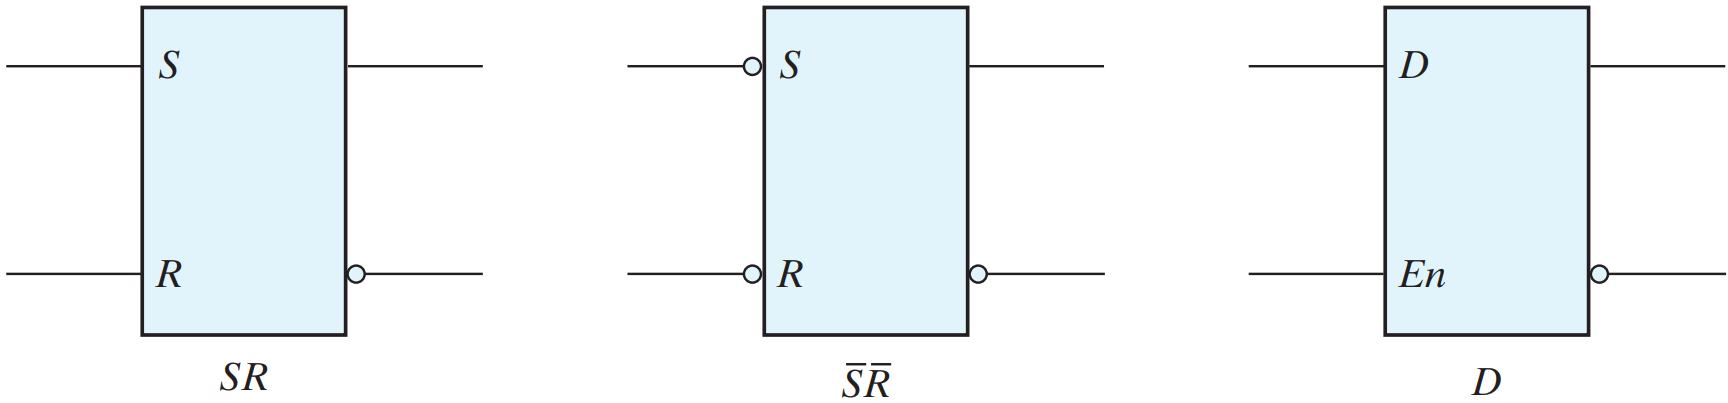
\includegraphics[width=\linewidth]{img/fig-5.7.png}
  \caption{Graphic symbols for latches}
  \label{fig:5.7}
\end{figure}

\begin{practice}{Practice Exercise 5.3}
Describe the functionality of a transparent latch. \\

\textbf{Answer:}
A transparent latch has a data input, an enable input, and output. When the enable input is asserted, the output of the latch follows the input to the latch. When the enable input is de-asserted, the output of the latch is held at the value that was present at the moment the enable input was de-asserted.
\end{practice}
